% Provenance (never printed): cycle 4 SVT, "La planete Terre": the history of
% the Earth read in the rocks, relative dating (superposition, recoupement,
% inclusion, continuite paleontologique), the ages of the Earth, eras and
% periods, the scale of geological time; see sources/book1/PROVENANCE.md.
% Book 1, grade 7, chapter 5.
% Vocabulary guard: owns relative dating / absolute age, the four principles,
% unconformity, era and geological period, the geological time scale. The
% method of radiometric dating is the physics books' and grade 12's: told
% here in two sentences, never defined. Fossils as evidence of evolution are
% the biology books' (one sentence of prose). "Ice age" is grade 8's: not used.
\chapter{Las edades de la Tierra}\label{ch:g7:geological-time}

En junio de 1788, el geólogo escocés James Hutton y dos amigos, el
matemático John Playfair y el químico James Hall, visitaron Siccar Point,
un promontorio rocoso ``lavado hasta quedar desnudo por el \omterm{def:g2:water-on-earth:ocean}{mar}'' en la
\omterm{def:g1:landscapes-around-us:water}{costa} de Escocia. En la base de la \omterm{def:g3:stones-pebbles-sand:rock}{roca} vieron capas grises puestas de
canto, casi verticales. Encima había capas de arenisca roja, suavemente
inclinadas. Hutton explicó lo que había ocurrido: las capas grises se
habían depositado horizontales en el fondo de un \omterm{def:g2:water-on-earth:ocean}{mar}, después se habían
levantado hasta ponerse de canto, después se habían desgastado, y solo
entonces se depositó encima la \omterm{def:g3:stones-pebbles-sand:sand}{arena} roja. Cada una de estas etapas
necesitó un tiempo inmenso. Playfair escribió más tarde: ``La mente parecía
sentir vértigo al mirar tan lejos en el abismo del tiempo''.
% ledger: ncse:siccar-point

\begin{omfigure}
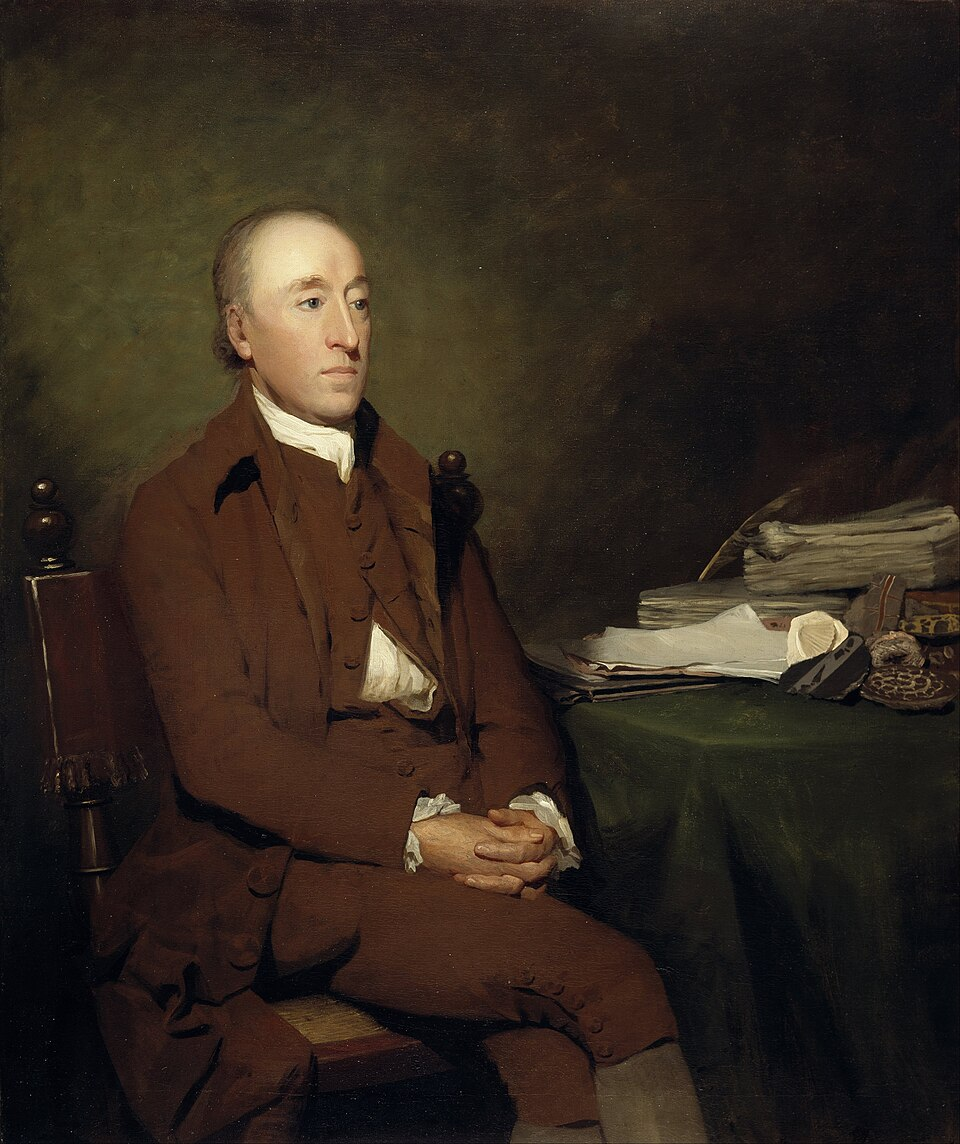
\includegraphics[width=0.3\linewidth]{images/book1/g7-hutton.jpg}

{\small James Hutton (1726--1797), pintado por Henry Raeburn. Hutton veía
en cada capa un lapso de \omterm{def:g1:watching-the-weather:weather}{tiempo}, con la más antigua abajo dondequiera que
las capas no se hayan dado la vuelta. Retrato de dominio público, vía Wikimedia Commons.}
% ledger: commons:hutton-portrait, usgs:hutton-smith
\label{fig:g7:geological-time:hutton}
\end{omfigure}

¿Cómo podemos saber qué \omterm{def:g3:stones-pebbles-sand:rock}{roca} es más antigua que otra, si no lleva ninguna
fecha escrita? ¿Qué edad tiene la Tierra? ¿Y cómo puede uno siquiera
imaginarse una historia tan larga?

\begin{recall}
Los \omterm{def:g7:sediments-and-fossils:sediment}{sedimentos} se depositan en capas, unas encima de otras, y se endurecen
hasta formar \omterm{def:g6:rocks-and-minerals:rock-families}{roca sedimentaria}; los \omterm{def:g7:sediments-and-fossils:fossil}{fósiles} son los restos o las huellas
de seres vivos conservados en una \omterm{def:g3:stones-pebbles-sand:rock}{roca} (\cref{ch:g7:sediments-and-fossils}).
Una \emph{\omterm{def:g7:earthquakes:fault}{falla}} es una rotura de las \omterm{def:g3:stones-pebbles-sand:rock}{rocas} a lo largo de la cual los dos
lados se han desplazado (\cref{ch:g7:earthquakes}). El granito es una
\emph{\omterm{def:g6:rocks-and-minerals:rock-families}{roca ígnea}}: se forma cuando la \omterm{def:g3:stones-pebbles-sand:rock}{roca} fundida se enfría lentamente, en
las profundidades; el esquisto es una \emph{\omterm{def:g6:rocks-and-minerals:rock-families}{roca metamórfica}}, transformada
por el calor y la presión; un conglomerado es una \omterm{def:g6:rocks-and-minerals:rock-families}{roca sedimentaria} hecha
de \omterm{def:g3:stones-pebbles-sand:pebble}{cantos rodados} cementados (\cref{ch:g6:rocks-and-minerals}).
\end{recall}

\section{¿Qué fue primero?}

Los historiadores pueden ordenar los acontecimientos incluso sin sus
fechas. La Primera Guerra Mundial fue antes que la Segunda: sus nombres lo
dicen. La televisión todavía no estaba en los hogares cuando los hermanos
Wright volaron por primera vez, en 1903, pero mucha gente vio los primeros
pasos en la Luna por televisión en 1969: así que primero fue el vuelo,
después la televisión en los hogares y después la Luna. Basta con reunir
pistas y compararlas para encontrar el orden. Para casi toda la historia de
la Tierra no hay ningún registro escrito, y los geólogos trabajan de la
misma manera: usan pistas conservadas en las \omterm{def:g3:stones-pebbles-sand:rock}{rocas}.
% ledger: usgs:events-order

\begin{definition}[Datación relativa y edad absoluta]\label{def:g7:geological-time:relative-dating}
La \emph{datación relativa}\index{datacion relativa@datación relativa}
ordena las \omterm{def:g3:stones-pebbles-sand:rock}{rocas} y los acontecimientos, del más antiguo al más reciente,
sin decir hace cuántos años ocurrieron: esta \omterm{def:g3:stones-pebbles-sand:rock}{roca} es más antigua que
aquella. Una \emph{edad absoluta}\index{edad absoluta} es una edad dada
como un número de años, por ejemplo ``\num{300} millones de años''.
\end{definition}

\section{Cuatro principios para ordenar las rocas}

Cuatro principios sencillos hacen la mayor parte del trabajo de la \omterm{def:g7:geological-time:relative-dating}{datación
relativa}. Están representados abajo, en cuatro acantilados imaginarios. El
primero lo enunció Nicolás Steno en 1669; Hutton se basó en él a finales del siglo~XVIII.
% ledger: usgs:hutton-smith, og:stratigraphy-principles

\begin{omfigure}
\tikzset{
  trilo/.pic={\fill[black!65] (0,0) ellipse (0.13 and 0.085);
              \draw[white, line width=0.3pt] (-0.11,0.028) -- (0.11,0.028) (-0.11,-0.028) -- (0.11,-0.028);},
  ammo/.pic={\draw[black!75, line width=0.45pt] (0,0) circle (0.1) (0,0) circle (0.062) (0,0) circle (0.028);}
}
\begin{minipage}[t]{0.49\linewidth}\centering
\begin{tikzpicture}[font=\footnotesize]
  \fill[lith sandstone] (0,0) rectangle (4.4,0.6);
  \fill[lith shale] (0,0.6) rectangle (4.4,1.2);
  \fill[lith limestone] (0,1.2) rectangle (4.4,1.8);
  \fill[lith sandstone] (0,1.8) rectangle (4.4,2.4);
  \foreach \k in {1,2,3,4} \node[fill=white, inner sep=1pt] at (0.35,0.6*\k-0.3) {\k};
  \draw (0,0) rectangle (4.4,2.4);
  \foreach \y in {0.6,1.2,1.8} \draw[contact] (0,\y) -- (4.4,\y);
  \draw[-{Stealth}, line width=0.8pt] (4.75,0.1) -- (4.75,2.3);
  \node[anchor=west] at (4.85,2.2) {más reciente};
  \node[anchor=west] at (4.85,0.2) {más antigua};
\end{tikzpicture}

{\small (a) Superposición: la capa 1 se formó primero, y la capa 4, la última.}
\end{minipage}\hfill
\begin{minipage}[t]{0.49\linewidth}\centering
\begin{tikzpicture}[font=\footnotesize]
  % left block, below the fault
  \begin{scope}
    \clip (0,0) -- (3.75,0) -- (3.25,2.4) -- (0,2.4) -- cycle;
    \fill[lith sandstone] (0,0) rectangle (5,0.6);
    \fill[lith shale] (0,0.6) rectangle (5,1.2);
    \fill[lith limestone] (0,1.2) rectangle (5,1.8);
    \fill[lith granite] (1.2,0) -- (1.85,0) -- (1.75,0.9) -- (1.9,1.8) -- (1.15,1.8) -- (1.3,0.9) -- cycle;
    \fill[lith sandstone] (0,1.8) rectangle (5,2.4);
    \foreach \y in {0.6,1.2} {\draw[contact] (0,\y) -- (1.25,\y); \draw[contact] (1.8,\y) -- (5,\y);}
    \draw[contact] (1.2,0) -- (1.3,0.9) -- (1.15,1.8) (1.85,0) -- (1.75,0.9) -- (1.9,1.8);
    \draw[contact] (0,1.8) -- (5,1.8);
  \end{scope}
  % right block, moved down along the fault
  \begin{scope}
    \clip (3.75,0) -- (5,0) -- (5,2.05) -- (3.32,2.05) -- cycle;
    \fill[lith sandstone] (3,-0.35) rectangle (5,0.25);
    \fill[lith shale] (3,0.25) rectangle (5,0.85);
    \fill[lith limestone] (3,0.85) rectangle (5,1.45);
    \fill[lith sandstone] (3,1.45) rectangle (5,2.05);
    \foreach \y in {0.25,0.85,1.45} \draw[contact] (3,\y) -- (5,\y);
  \end{scope}
  \draw (0,0) -- (5,0) -- (5,2.05) -- (3.32,2.05) (3.25,2.4) -- (0,2.4) -- (0,0);
  \draw[fault] (3.75,0) -- (3.25,2.4);
  \node[anchor=south, fill=white, inner sep=1pt] at (1.5,2.45) {granito};
  \draw[black!70] (1.5,2.45) -- (1.52,1.6);
  \node[anchor=south] at (4.2,2.45) {falla};
  \draw[black!70] (4.0,2.45) -- (3.4,1.75);
\end{tikzpicture}

{\small (b) Intersección: el granito es más reciente que las tres capas que
corta, y más antiguo que la capa de arriba; la \omterm{def:g7:earthquakes:fault}{falla}, que las rompe todas,
es lo más reciente.}
\end{minipage}

\bigskip
\begin{minipage}[t]{0.49\linewidth}\centering
\begin{tikzpicture}[font=\footnotesize]
  \fill[lith granite] (0,0) -- (4.4,0) -- (4.4,1.05) .. controls (3.4,0.95) and (2.6,1.2) .. (1.6,1.0) .. controls (0.9,0.88) and (0.4,1.1) .. (0,1.0) -- cycle;
  \fill[lith conglomerate] (0,2.4) -- (4.4,2.4) -- (4.4,1.05) .. controls (3.4,0.95) and (2.6,1.2) .. (1.6,1.0) .. controls (0.9,0.88) and (0.4,1.1) .. (0,1.0) -- cycle;
  \foreach \x/\y/\a/\b in {0.5/1.35/0.2/0.12, 1.3/1.25/0.16/0.1, 2.1/1.45/0.22/0.13, 2.9/1.3/0.17/0.11, 3.7/1.4/0.2/0.12, 0.9/1.8/0.15/0.1, 2.5/1.95/0.17/0.1, 3.4/1.85/0.14/0.09}
    \filldraw[fill=omLithGranite, draw=black!70, line width=0.3pt] (\x,\y) ellipse [x radius=\a, y radius=\b];
  \draw[unconformity] (0,1.0) .. controls (0.4,1.1) and (0.9,0.88) .. (1.6,1.0) .. controls (2.6,1.2) and (3.4,0.95) .. (4.4,1.05);
  \draw (0,0) rectangle (4.4,2.4);
  \node[fill=white, inner sep=1pt] at (2.2,0.45) {granito};
  \node[anchor=west] at (4.5,1.7) {conglomerado};
  \node[anchor=west, align=left] at (4.5,1.15) {cantos de\\granito};
  \draw[black!70] (4.5,1.15) -- (3.85,1.4);
\end{tikzpicture}

{\small (c) Inclusión: los \omterm{def:g3:stones-pebbles-sand:pebble}{cantos} de granito son más antiguos que el
conglomerado que los contiene.}
\end{minipage}\hfill
\begin{minipage}[t]{0.49\linewidth}\centering
\begin{tikzpicture}[font=\footnotesize]
  % place A
  \fill[lith shale] (0,0) rectangle (1.3,0.8);
  \fill[lith limestone] (0,0.8) rectangle (1.3,1.6);
  \fill[lith sandstone] (0,1.6) rectangle (1.3,2.4);
  \draw (0,0) rectangle (1.3,2.4); \draw[contact] (0,0.8) -- (1.3,0.8) (0,1.6) -- (1.3,1.6);
  \foreach \x in {0.3,0.65,1.0} {\pic at (\x,0.4) {trilo}; \pic at (\x,1.2) {ammo};}
  \node[anchor=south] at (0.65,2.45) {lugar A};
  % place B
  \fill[lith sandstone] (3.6,0.4) rectangle (4.9,1.0);
  \fill[lith shale] (3.6,1.0) rectangle (4.9,2.0);
  \fill[lith limestone] (3.6,0) rectangle (4.9,0.4);
  \draw (3.6,0) rectangle (4.9,2.0); \draw[contact] (3.6,0.4) -- (4.9,0.4) (3.6,1.0) -- (4.9,1.0);
  \foreach \x in {3.9,4.25,4.6} {\pic at (\x,0.7) {trilo}; \pic at (\x,1.5) {ammo};}
  \node[anchor=south] at (4.25,2.45) {lugar B};
  \draw[dashed, black!70] (1.3,0.8) -- (3.6,1.0) (1.3,0) -- (3.6,0.4) (1.3,1.6) -- (3.6,2.0);
  \pic at (2.15,-0.3) {trilo}; \node[anchor=west] at (2.3,-0.3) {trilobites};
  \pic at (2.15,2.3) {ammo}; \node[anchor=west] at (2.3,2.3) {amonites};
\end{tikzpicture}

{\small (d) Sucesión faunística: las capas con los mismos \omterm{def:g7:sediments-and-fossils:fossil}{fósiles} tienen la
misma edad, aunque sus \omterm{def:g3:stones-pebbles-sand:rock}{rocas} sean distintas.}
\end{minipage}

\medskip
{\small Los cuatro principios de la \omterm{def:g7:geological-time:relative-dating}{datación relativa}, en cuatro acantilados
imaginarios.}
% ledger: usgs:hutton-smith, usgs:cross-cutting, nps:cross-cutting, eli:relative-dating, usgs:fossil-succession
\label{fig:g7:geological-time:principles}
\end{omfigure}

\begin{definition}[Principio de superposición]\label{def:g7:geological-time:superposition}
El \emph{principio de superposición}\index{superposicion, principio de@superposición, principio de}:
en un montón de \omterm{def:g7:sediments-and-fossils:layer}{capas sedimentarias} que no se ha dado la vuelta, cada
capa es más reciente que la capa de debajo y más antigua que la de encima.
La capa más antigua está abajo, y la más reciente, arriba.
\end{definition}
% ledger: usgs:hutton-smith, eli:relative-dating

\begin{definition}[Principio de intersección]\label{def:g7:geological-time:cross-cutting}
El \emph{principio de intersección}\index{interseccion, principio de@intersección, principio de}: una \omterm{def:g3:stones-pebbles-sand:rock}{roca} o una estructura que corta otras \omterm{def:g3:stones-pebbles-sand:rock}{rocas}
es más reciente que las \omterm{def:g3:stones-pebbles-sand:rock}{rocas} que corta. Una masa de granito que atraviesa
unas capas, una \omterm{def:g7:earthquakes:fault}{falla} que las rompe y una superficie de \omterm{def:g5:water-shapes-the-land:erosion}{erosión} que las
desgasta son todas más recientes que esas capas.
\end{definition}
% ledger: usgs:cross-cutting, nps:cross-cutting, eli:relative-dating

\begin{definition}[Principio de inclusión]\label{def:g7:geological-time:inclusion}
El \emph{principio de inclusión}\index{inclusion, principio de@inclusión, principio de}: los trozos de
una \omterm{def:g3:stones-pebbles-sand:rock}{roca} que se encuentran dentro de otra \omterm{def:g3:stones-pebbles-sand:rock}{roca} son más antiguos que la
\omterm{def:g3:stones-pebbles-sand:rock}{roca} que los contiene. Los \omterm{def:g3:stones-pebbles-sand:pebble}{cantos} de un conglomerado existían antes de que
el conglomerado se formara a su alrededor.
\end{definition}
% ledger: eli:relative-dating

\begin{definition}[Principio de sucesión faunística]\label{def:g7:geological-time:fossil-succession}
El \emph{principio de sucesión faunística}\index{sucesion faunistica, principio de@sucesión faunística, principio de}: las clases de animales y de plantas que se encuentran como \omterm{def:g7:sediments-and-fossils:fossil}{fósiles} cambian
de las capas más antiguas a las más recientes, siempre en el mismo orden.
Las \omterm{def:g3:stones-pebbles-sand:rock}{rocas} que contienen las mismas clases de \omterm{def:g7:sediments-and-fossils:fossil}{fósiles} tienen la misma edad,
aunque estén muy lejos unas de otras.
\end{definition}
% ledger: usgs:fossil-succession


El \omterm{def:g7:geological-time:superposition}{principio de superposición} solo vale para las capas que no se han dado
la vuelta: en unos pocos lugares, la formación de las \omterm{def:g1:landscapes-around-us:landform}{montañas} ha plegado
un montón de capas con tanta fuerza que ha quedado del revés. Los geólogos
buscan entonces pistas que muestren en qué sentido se formaron las capas
--- las huellas de pisadas y las rizaduras, por ejemplo, están en la cara
superior de una capa. El \omterm{def:g7:geological-time:fossil-succession}{principio de sucesión faunística} funciona porque
la vida en la Tierra ha cambiado con el tiempo: la mayoría de los \omterm{def:g7:sediments-and-fossils:fossil}{fósiles}
pertenecen a especies que ya no viven en ninguna parte. Por qué cambió la
vida se cuenta en los libros de biología.
% ledger: eli:relative-dating, usgs:fossil-succession, nps:ripple-marks

\begin{history}[William Smith, el constructor de canales]
Entre 1785 y 1800, mientras Hutton trabajaba en Escocia, William Smith, un
ingeniero inglés que construía canales, recogió las conchas \omterm{def:g7:sediments-and-fossils:fossil}{fósiles} de las
calizas y lutitas que excavaba. Descubrió que cada capa tenía sus propios
\omterm{def:g7:sediments-and-fossils:fossil}{fósiles}, distintos de los de las capas de encima y de debajo. Usando esos
\omterm{def:g7:sediments-and-fossils:fossil}{fósiles} como marcadores, podía reconocer la misma capa allí donde
apareciera, y dibujó algunos de los primeros \omterm{def:g2:drawing-to-map:map}{mapas} geológicos de grandes
regiones.
\end{history}
% ledger: usgs:hutton-smith

\section{Huecos en el registro}

En Siccar Point, las capas grises y la arenisca roja no se formaron una
detrás de otra. Entre ambas, las capas grises se inclinaron y se
levantaron, y después se desgastaron durante muchísimo tiempo, y no se
conservó ninguna capa de esa época. La superficie que separa los dos
conjuntos de \omterm{def:g3:stones-pebbles-sand:rock}{rocas} es un hueco en el registro.

\begin{definition}[Discordancia]\label{def:g7:geological-time:unconformity}
Una \emph{discordancia}\index{discordancia} es una superficie de \omterm{def:g5:water-shapes-the-land:erosion}{erosión}
entre dos conjuntos de \omterm{def:g3:stones-pebbles-sand:rock}{rocas} formados en épocas muy distintas: las \omterm{def:g3:stones-pebbles-sand:rock}{rocas}
más antiguas se desgastaron antes de que las más recientes se depositaran
encima. Señala un largo tiempo del que no se ha conservado ninguna capa.
\end{definition}
% ledger: ncse:siccar-point, eli:relative-dating

\begin{omfigure}
\begin{tikzpicture}[font=\footnotesize, x=1cm, y=1cm]
  \def\stripes#1#2#3{% x0, width, top: vertical layers
    \foreach \i in {0,...,7} {
      \pgfmathsetmacro{\xa}{#1+\i*#2/8}
      \pgfmathsetmacro{\xb}{#1+(\i+1)*#2/8}
      \ifodd\i\def\lithc{omLithSchist}\else\def\lithc{omLithShale}\fi
      \fill[\lithc] (\xa,0) rectangle (\xb,#3);
      \draw[black!55, line width=0.3pt] (\xa,0) -- (\xa,#3);
    }}
  % 1: flat layers under the sea
  \fill[omSea!70] (0,1.6) rectangle (3.4,2.4);
  \foreach \k in {0,...,3} {
    \ifodd\k\def\lithc{omLithSchist}\else\def\lithc{omLithShale}\fi
    \fill[\lithc] (0,0.4*\k) rectangle (3.4,0.4*\k+0.4);
    \draw[black!55, line width=0.3pt] (0,0.4*\k) -- (3.4,0.4*\k);
  }
  \draw (0,0) rectangle (3.4,2.4);
  \node[anchor=north, align=center] at (1.7,-0.1) {1. Capas depositadas\\horizontales en un mar};
  % 2: pushed up on end
  \begin{scope}[xshift=3.9cm]
    \begin{scope}
      \clip (0,0) -- (3.4,0) -- (3.4,1.7) -- (2.6,2.2) -- (1.6,1.75) -- (0.9,2.3) -- (0,1.8) -- cycle;
      \stripes{0}{3.4}{2.4}
    \end{scope}
    \draw (0,1.8) -- (0.9,2.3) -- (1.6,1.75) -- (2.6,2.2) -- (3.4,1.7);
    \draw (0,1.8) -- (0,0) -- (3.4,0) -- (3.4,1.7);
    \node[anchor=north, align=center] at (1.7,-0.1) {2. Puestas de canto,\\levantadas sobre el mar};
  \end{scope}
  % 3: worn flat
  \begin{scope}[xshift=7.8cm]
    \stripes{0}{3.4}{1.3}
    \draw[unconformity] (0,1.3) -- (3.4,1.3);
    \draw (0,1.3) -- (0,0) -- (3.4,0) -- (3.4,1.3);
    \node[anchor=north, align=center] at (1.7,-0.1) {3. Desgastadas\\durante mucho tiempo};
  \end{scope}
  % 4: new layers on top
  \begin{scope}[xshift=11.7cm]
    \stripes{0}{3.4}{1.3}
    \fill[om lith={red!22}{om sand}] (0,1.3) rectangle (3.4,1.85);
    \fill[om lith={red!30}{om sand}] (0,1.85) rectangle (3.4,2.4);
    \draw[contact] (0,1.85) -- (3.4,1.85);
    \draw[unconformity, line width=0.9pt] (0,1.3) -- (3.4,1.3);
    \draw (0,0) rectangle (3.4,2.4);
    \node[anchor=north, align=center] at (1.7,-0.1) {4. Capas nuevas encima:\\una discordancia};
  \end{scope}
  \foreach \x in {3.45,7.35,11.25} \draw[-{Stealth}, line width=0.7pt] (\x,1.2) -- (\x+0.4,1.2);
\end{tikzpicture}

{\small Cómo se forma una \omterm{def:g7:geological-time:unconformity}{discordancia} como la de Siccar Point. La línea
ondulada es la \omterm{def:g7:geological-time:unconformity}{discordancia}: el largo tiempo de las etapas 2 y 3 no dejó
ninguna capa.}
% ledger: ncse:siccar-point
\label{fig:g7:geological-time:unconformity}
\end{omfigure}

\section{Leer la historia de una región}

Un corte geológico muestra las \omterm{def:g3:stones-pebbles-sand:rock}{rocas} tal como aparecerían en un corte
vertical hecho en el suelo. Los cuatro principios lo convierten en una
historia.

\begin{method}[Ordenar los acontecimientos de un corte geológico]\label{met:g7:geological-time:ordering}
\begin{enumerate}
  \item Busca las \omterm{def:g3:stones-pebbles-sand:rock}{rocas} más antiguas: las que todo lo demás corta, o las
        que están en la base del montón.
  \item Busca cada \omterm{def:g3:stones-pebbles-sand:rock}{roca} o estructura que corta a otras (un granito, una
        \omterm{def:g7:earthquakes:fault}{falla}, una superficie de \omterm{def:g5:water-shapes-the-land:erosion}{erosión}): es más reciente que todo lo que
        corta.
  \item Lee las capas de abajo arriba (superposición) y busca las
        \omterm{def:g7:geological-time:unconformity}{discordancias}, donde falta tiempo.
  \item Las capas se depositan horizontales: si están inclinadas o
        plegadas, el plegamiento llegó después.
  \item Escribe los acontecimientos en orden, del más antiguo al más
        reciente, con la pista de cada uno.
\end{enumerate}
\end{method}
% ledger: eli:relative-dating, usgs:cross-cutting, nps:cross-cutting

\begin{omfigure}
\begin{tikzpicture}
\begin{axis}[x=1.4cm, y=0.007cm, xmin=0, xmax=10, ymin=-500, ymax=300,
  axis on top, tick label style={font=\scriptsize}, label style={font=\small},
  xlabel={distancia hacia el este desde E (km)}, ylabel={altura (m)},
  ytick={-400,-200,0,200}, clip mode=individual]
\addplot[lith schist, draw=black, line width=0.3pt, even odd rule] table {figdata/out/grade-7-varden_history-unit-schist.dat};
\addplot[lith granite, draw=black, line width=0.3pt, even odd rule] table {figdata/out/grade-7-varden_history-unit-granite.dat};
\addplot[om lith={icsTriassic!35}{om sand}, draw=black, line width=0.3pt, even odd rule] table {figdata/out/grade-7-varden_history-unit-sandstone.dat};
\addplot[om lith={icsJurassic!40}{om limestone}, draw=black, line width=0.3pt, even odd rule] table {figdata/out/grade-7-varden_history-unit-limestone.dat};
\addplot[om lith={icsJurassic!15}{om shale}, draw=black, line width=0.3pt, even odd rule] table {figdata/out/grade-7-varden_history-unit-shale.dat};
\addplot[om lith={icsCretaceous!35}{om limestone}, draw=black, line width=0.3pt, even odd rule] table {figdata/out/grade-7-varden_history-unit-chalk.dat};
\addplot[lith alluvium, draw=black, line width=0.3pt, even odd rule] table {figdata/out/grade-7-varden_history-unit-alluvium.dat};
\addplot[omThm, line width=1.3pt] table {figdata/out/grade-7-varden_history-base.dat};
\addplot[black, line width=0.8pt] table {figdata/out/grade-7-varden_history-ground.dat};
\addplot[fault, line width=1.3pt] table {figdata/out/grade-7-varden_history-fault.dat};
\node[font=\small, above right] at (axis cs:0,300) {E (oeste)};
\node[font=\small, above left] at (axis cs:10,300) {F (este)};
\end{axis}
\end{tikzpicture}

\smallskip
{\small\setlength{\tabcolsep}{4pt}
\begin{tabular}{@{}llll@{}}
\tikz\fill[lith schist, draw=black] (0,0) rectangle (0.5,0.3); esquisto &
\tikz\fill[lith granite, draw=black] (0,0) rectangle (0.5,0.3); granito &
\tikz\fill[om lith={icsTriassic!35}{om sand}, draw=black] (0,0) rectangle (0.5,0.3); arenisca &
\tikz\fill[om lith={icsJurassic!40}{om limestone}, draw=black] (0,0) rectangle (0.5,0.3); caliza \\
\tikz\fill[om lith={icsJurassic!15}{om shale}, draw=black] (0,0) rectangle (0.5,0.3); lutita &
\tikz\fill[om lith={icsCretaceous!35}{om limestone}, draw=black] (0,0) rectangle (0.5,0.3); creta &
\tikz\fill[lith alluvium, draw=black] (0,0) rectangle (0.5,0.3); \omterm{def:g3:stones-pebbles-sand:sand}{arena} de \omterm{def:g1:landscapes-around-us:water}{río} &
\tikz\draw[omThm, line width=1.3pt] (0,0.15) -- (0.5,0.15); base de la arenisca \\
\end{tabular}}

\smallskip
{\small Corte E--F, de oeste (E) a este (F), a través del centro de las
Colinas de Varden, la región inventada de esta serie, pasando por su
granito. La línea negra gruesa es la \omterm{def:g7:earthquakes:fault}{falla}. Las alturas están
multiplicadas por 5 respecto a las distancias, para que las capas se vean
mejor.}
% ledger: (invented region: figdata/shared/region.py, section E--F by figdata/grade-7/varden_history.py)
\label{fig:g7:geological-time:section}
\end{omfigure}

\begin{example}[La historia de las Colinas de Varden]\label{ex:g7:geological-time:varden}
Apliquemos el método al corte E--F.
\begin{enumerate}
  \item El granito corta el esquisto, que está bajo todas las capas: es
        la \omterm{def:g3:stones-pebbles-sand:rock}{roca} más antigua.
  \item El granito corta el esquisto (intersección), así que es más
        reciente. No corta ninguna de las capas de encima: es más antiguo
        que la arenisca.
  \item El granito se enfrió en las profundidades, y sin embargo la base
        de la arenisca, que descansa sobre el esquisto, llega hasta el
        techo del granito: las \omterm{def:g3:stones-pebbles-sand:rock}{rocas} que los cubrían se desgastaron antes
        de que llegara la \omterm{def:g3:stones-pebbles-sand:sand}{arena}. La base de la arenisca es una
        \omterm{def:g7:geological-time:unconformity}{discordancia}.
  \item La arenisca, la caliza, la lutita y la creta se depositaron en ese
        orden (superposición).
  \item Las capas se depositaron horizontales, pero ahora están plegadas,
        arqueadas hacia arriba sobre el granito y dobladas hacia abajo más
        al este: el plegamiento llegó después de la creta.
  \item La \omterm{def:g7:earthquakes:fault}{falla} rompe todas las capas plegadas: es más reciente que el
        plegamiento.
  \item La superficie actual del suelo lo corta todo, y la \omterm{def:g3:stones-pebbles-sand:sand}{arena} de \omterm{def:g1:landscapes-around-us:water}{río}
        descansa encima: la \omterm{def:g5:water-shapes-the-land:erosion}{erosión} y los \omterm{def:g1:landscapes-around-us:water}{ríos} son los acontecimientos más
        recientes.
\end{enumerate}
La historia, empezando por lo más antiguo: el esquisto; el granito; la
\omterm{def:g5:water-shapes-the-land:erosion}{erosión}; las cuatro capas; el plegamiento; la \omterm{def:g7:earthquakes:fault}{falla}; la \omterm{def:g5:water-shapes-the-land:erosion}{erosión} actual y
la \omterm{def:g3:stones-pebbles-sand:sand}{arena} de \omterm{def:g1:landscapes-around-us:water}{río}.
% ledger: (invented region: figdata/grade-7/varden_history.py main table)
\end{example}

La \omterm{def:g7:geological-time:relative-dating}{datación relativa} da el orden de los acontecimientos, pero no sus
fechas ni cuánto duró cada uno: el método dice que la \omterm{def:g7:earthquakes:fault}{falla} es más
reciente que la creta, no cuántos años más.

\section{Eras y periodos}

La sucesión faunística permite a los geólogos relacionar capas de todo el
mundo. Reuniendo sus observaciones, dividieron la historia de la Tierra en
intervalos de tiempo, del mismo modo que los historiadores hablan de siglos
y de reinados.
% ledger: usgs:hutton-smith, usgs:fossil-succession

\begin{omfigure}
\begin{tikzpicture}[font=\footnotesize]
\begin{axis}[name=long, x dir=reverse, xmin=0, xmax=4600, ymin=0, ymax=1,
  width=14.3cm, height=1.7cm, scale only axis, axis y line=none, axis x line*=bottom,
  xtick={4500,4000,3000,2000,1000}, tick label style={font=\scriptsize}, clip=false]
  \pgfplotsinvokeforeach{Hadean,Archean,Proterozoic,Phanerozoic}{
    \addplot[fill=ics#1, draw=black!70, line width=0.3pt] table {figdata/out/grade-7-time_scale-bar-#1.dat};}
  \node[anchor=center, font=\scriptsize, fill=white, fill opacity=0.85, text opacity=1, inner sep=1pt] at (axis cs:4299,0.5) {Hádico};
  \node[anchor=center, font=\scriptsize, fill=white, fill opacity=0.85, text opacity=1, inner sep=1pt] at (axis cs:3265.5,0.5) {Arcaico};
  \node[anchor=center, font=\scriptsize, fill=white, fill opacity=0.85, text opacity=1, inner sep=1pt] at (axis cs:1519.4,0.5) {Proterozoico};
  \node[anchor=center, font=\scriptsize, fill=white, fill opacity=0.85, text opacity=1, inner sep=1pt] at (axis cs:269.4,0.5) {Fanerozoico};
  \coordinate (z1) at (axis cs:538.8,0);
  \coordinate (z2) at (axis cs:0,0);
\end{axis}
\begin{axis}[at={(long.south west)}, anchor=north west, yshift=-1.3cm,
  x dir=reverse, xmin=0, xmax=540, ymin=0, ymax=3.2,
  width=14.3cm, height=3.6cm, scale only axis, axis y line=none, axis x line*=bottom,
  xtick={500,400,300,200,100,0}, tick label style={font=\scriptsize},
  xlabel={millones de años atrás}, label style={font=\small}, clip=false]
  \pgfplotsinvokeforeach{Paleozoic,Mesozoic,Cenozoic}{
    \addplot[fill=ics#1, draw=black!70, line width=0.3pt] table[x=age, y expr=2.4+0.8*\thisrow{y}] {figdata/out/grade-7-time_scale-bar-#1.dat};}
  \pgfplotsinvokeforeach{Cambrian,Ordovician,Silurian,Devonian,Carboniferous,Permian,Triassic,Jurassic,Cretaceous,Paleogene,Neogene,Quaternary}{
    \addplot[fill=ics#1, draw=black!70, line width=0.3pt] table[x=age, y expr=2.4*\thisrow{y}] {figdata/out/grade-7-time_scale-bar-#1.dat};}
  \node[anchor=center, font=\footnotesize\bfseries, fill=white, fill opacity=0.85, text opacity=1, inner sep=1pt] at (axis cs:395.351,2.8) {Paleozoico};
  \node[anchor=center, font=\footnotesize\bfseries, fill=white, fill opacity=0.85, text opacity=1, inner sep=1pt] at (axis cs:158.951,2.8) {Mesozoico};
  \node[anchor=center, font=\footnotesize\bfseries, fill=white, fill opacity=0.85, text opacity=1, inner sep=1pt] at (axis cs:33,2.8) {Cenozoico};
  \node[anchor=center, rotate=90, font=\scriptsize, fill=white, fill opacity=0.85, text opacity=1, inner sep=1pt] at (axis cs:512.825,1.2) {Cámbrico};
  \node[anchor=center, rotate=90, font=\scriptsize, fill=white, fill opacity=0.85, text opacity=1, inner sep=1pt] at (axis cs:464.975,1.2) {Ordovícico};
  \node[anchor=center, rotate=90, font=\scriptsize, fill=white, fill opacity=0.85, text opacity=1, inner sep=1pt] at (axis cs:431.36,1.2) {Silúrico};
  \node[anchor=center, rotate=90, font=\scriptsize, fill=white, fill opacity=0.85, text opacity=1, inner sep=1pt] at (axis cs:389.24,1.2) {Devónico};
  \node[anchor=center, rotate=90, font=\scriptsize, fill=white, fill opacity=0.85, text opacity=1, inner sep=1pt] at (axis cs:328.88,1.2) {Carbonífero};
  \node[anchor=center, rotate=90, font=\scriptsize, fill=white, fill opacity=0.85, text opacity=1, inner sep=1pt] at (axis cs:275.401,1.2) {Pérmico};
  \node[anchor=center, rotate=90, font=\scriptsize, fill=white, fill opacity=0.85, text opacity=1, inner sep=1pt] at (axis cs:226.651,1.2) {Triásico};
  \node[anchor=center, rotate=90, font=\scriptsize, fill=white, fill opacity=0.85, text opacity=1, inner sep=1pt] at (axis cs:172.25,1.2) {Jurásico};
  \node[anchor=center, rotate=90, font=\scriptsize, fill=white, fill opacity=0.85, text opacity=1, inner sep=1pt] at (axis cs:104.55,1.2) {Cretácico};
  \node[anchor=center, rotate=90, font=\scriptsize, fill=white, fill opacity=0.85, text opacity=1, inner sep=1pt] at (axis cs:44.52,1.2) {Paleógeno};
  \node[anchor=center, rotate=90, font=\scriptsize, fill=white, fill opacity=0.85, text opacity=1, inner sep=1pt] at (axis cs:12.81,1.2) {Neógeno};
  \node[anchor=west, xshift=3pt, font=\scriptsize] at (axis cs:1.29,1.2) {Cuaternario};
  \coordinate (w1) at (axis cs:540,3.2);
  \coordinate (w2) at (axis cs:0,3.2);
\end{axis}
\draw[dashed, black!60] (z1) -- ++(0,-0.5) -- (w1) (z2) -- (w2);
\end{tikzpicture}

{\small La \omterm{def:g7:geological-time:time-scale}{escala de tiempo geológico}, con los colores de la tabla
internacional. Arriba: toda la historia de la Tierra. Abajo: su última
parte, el Fanerozoico, ampliada: sus tres \omterm{def:g7:geological-time:era-period}{eras} y los doce \omterm{def:g7:geological-time:era-period}{periodos
geológicos}. Edades en millones de años antes de hoy.}
% ledger: ics:base.Hadean, ics:base.Archean, ics:base.Proterozoic, ics:base.Paleozoic, ics:base.Mesozoic, ics:base.Cenozoic, ics:colour.Hadean (figdata/grade-7/time_scale.py reads every ics base and colour row of the shared ledger)
\label{fig:g7:geological-time:scale}
\end{omfigure}

\begin{definition}[Era y periodo geológico]\label{def:g7:geological-time:era-period}
Una \emph{era}\index{era} es un intervalo largo de la historia de la
Tierra, definido por el tipo general de vida que existía en esa época: el
Paleozoico, el Mesozoico y el Cenozoico. Cada era se divide en intervalos
más cortos, los \emph{periodos geológicos}\index{periodo geologico@periodo geológico},
como el Jurásico o el Cretácico.
\end{definition}
% ledger: usgs:hutton-smith

\begin{definition}[Escala de tiempo geológico]\label{def:g7:geological-time:time-scale}
La \emph{escala de tiempo geológico}\index{escala de tiempo geologico@escala de tiempo geológico} es la lista
ordenada de las divisiones de la historia de la Tierra --- los largos
intervalos de su historia primitiva, las \omterm{def:g7:geological-time:era-period}{eras} y los \omterm{def:g7:geological-time:era-period}{periodos geológicos}
---, con la edad, en años, del comienzo de cada una. Una tabla
internacional da a cada división su nombre, su edad y su color.
\end{definition}
% ledger: ics:base.Hadean, ics:colour.Hadean


Las tres \omterm{def:g7:geological-time:era-period}{eras} son recientes comparadas con toda la historia. El Paleozoico
empezó hace \num{538.8} millones de años, cuando los \omterm{def:g7:sediments-and-fossils:fossil}{fósiles} de animales
con concha se volvieron frecuentes; el Mesozoico duró desde hace
\num{251.9} hasta hace \num{66} millones de años; el Cenozoico, la \omterm{def:g7:geological-time:era-period}{era} en
que vivimos, empezó hace \num{66} millones de años. Antes del Paleozoico
se extienden tres largos intervalos, el Hádico, el Arcaico y el
Proterozoico: cubren alrededor del 88~\% de la historia de la Tierra, y
sin embargo sus \omterm{def:g7:sediments-and-fossils:fossil}{fósiles} son raros. Los dinosaurios vivieron en el
Mesozoico: dominaron durante más de \num{100} millones de años, y al final
del Cretácico habían desaparecido todos.
% ledger: ics:base.Paleozoic, ics:base.Mesozoic, ics:base.Cenozoic, usgs:numeric-scale, usgs:dinosaurs-extinct (figdata/grade-7/time_scale.py main table: 88.1 %)

Las Colinas de Varden encajan en esta escala. Su arenisca es del Triásico;
su caliza y su lutita, del Jurásico; su creta, del Cretácico: las tres
pertenecen al Mesozoico. En el corte E--F están dibujadas con versiones
pálidas de los colores de la tabla.
% ledger: (invented region: figdata/shared/region.py UNITS)

\section{La historia de la Tierra en un año}

Los números en miles de millones de años son difíciles de imaginar.
Imagina, en cambio, toda la historia de la Tierra comprimida en un solo
año. La Tierra se forma el 1~de enero a medianoche; hoy son las doce en
punto de la noche del 31~de diciembre. La Tierra tiene unos \num{4540}
millones de años, así que un día de este año representa $4540 \div 365$,
unos \num{12.4} millones de años.
% ledger: usgs:age-earth (figdata/grade-7/earth_calendar.py)

\begin{omfigure}
\begin{tikzpicture}[font=\footnotesize]
\begin{axis}[xmin=0, xmax=365, ymin=0, ymax=1, width=15.2cm, height=0.9cm,
  scale only axis, axis y line=none, axis x line=none, clip=false]
  \addplot[ycomb, black!60, line width=0.4pt] table[x=day, y expr=1] {figdata/out/grade-7-earth_calendar-days.dat};
  \draw[black!70] (axis cs:0,0) rectangle (axis cs:365,1);
  \node[anchor=center, font=\scriptsize] at (axis cs:15.5,0.5) {ene};
  \node[anchor=center, font=\scriptsize] at (axis cs:45,0.5) {feb};
  \node[anchor=center, font=\scriptsize] at (axis cs:74.5,0.5) {mar};
  \node[anchor=center, font=\scriptsize] at (axis cs:105,0.5) {abr};
  \node[anchor=center, font=\scriptsize] at (axis cs:135.5,0.5) {may};
  \node[anchor=center, font=\scriptsize] at (axis cs:166,0.5) {jun};
  \node[anchor=center, font=\scriptsize] at (axis cs:196.5,0.5) {jul};
  \node[anchor=center, font=\scriptsize] at (axis cs:227.5,0.5) {ago};
  \node[anchor=center, font=\scriptsize] at (axis cs:258,0.5) {sep};
  \node[anchor=center, font=\scriptsize] at (axis cs:288.5,0.5) {oct};
  \node[anchor=center, font=\scriptsize] at (axis cs:319,0.5) {nov};
  \node[anchor=center, font=\scriptsize] at (axis cs:349.5,0.5) {dic};
  \addplot[only marks, mark=triangle*, mark size=2.6pt, omThm, mark options={rotate=180}]
    table[x=day, y expr=1.18] {figdata/out/grade-7-earth_calendar.dat};
  \node[anchor=west, rotate=40, xshift=2pt, yshift=4pt, font=\scriptsize] at (axis cs:0,1.18) {1 de enero: se forma la Tierra};
  \node[anchor=west, rotate=40, xshift=2pt, yshift=4pt, font=\scriptsize] at (axis cs:41,1.18) {11 de febrero: rocas más antiguas};
  \node[anchor=west, rotate=40, xshift=2pt, yshift=4pt, font=\scriptsize] at (axis cs:83.61,1.18) {25 de marzo: fósiles más antiguos};
  \node[anchor=east, rotate=-40, xshift=-2pt, yshift=4pt, font=\scriptsize] at (axis cs:321.68,1.18) {18 de noviembre: las conchas abundan};
  \node[anchor=east, rotate=-40, xshift=-2pt, yshift=4pt, font=\scriptsize] at (axis cs:359.69,1.18) {26 de diciembre: fin de los dinosaurios};
\end{axis}
\end{tikzpicture}

{\small La historia de la Tierra como un año del calendario: cada mes
representa unos \num{373} millones de años, y cada día, unos \num{12.4}
millones de años. Las fechas se calculan a partir de las edades de los
acontecimientos.}
% ledger: usgs:age-earth, usgs:oldest-rocks, usgs:numeric-scale, ics:base.Paleozoic, ics:base.Paleogene (figdata/grade-7/earth_calendar.py)
\label{fig:g7:geological-time:calendar}
\end{omfigure}

Las \omterm{def:g3:stones-pebbles-sand:rock}{rocas} más antiguas halladas hasta ahora llegan el 11~de febrero; los
\omterm{def:g7:sediments-and-fossils:fossil}{fósiles} más antiguos conocidos, el 25~de marzo. Durante la mayor parte del
año no hay animales con concha, y los \omterm{def:g7:sediments-and-fossils:fossil}{fósiles} son raros. Los animales con
concha solo se vuelven frecuentes el 18~de noviembre. Los dinosaurios,
tras más de \num{100} millones de años de dominio, han desaparecido el
26~de diciembre, cinco días antes de que acabe el año. Nuestra propia
especie llega en la última hora del 31~de diciembre: el problema de este
capítulo averigua cuándo.
% ledger: usgs:oldest-rocks, usgs:numeric-scale, ics:base.Paleozoic, ics:base.Paleogene, usgs:dinosaurs-extinct, hublin:jebel-irhoud

\begin{inthelab}[Una cinta del tiempo]
En el interior, desenrolla \qty{4.54}{m} de cinta de papel o de rollo de
caja registradora en el suelo de un pasillo: a \qty{1}{mm} por cada millón
de años, cabe en ella toda la historia de la Tierra. Marca el comienzo del
Paleozoico a \qty{54}{cm} del final, y el final de los dinosaurios a
\qty{6.6}{cm} del final. Después intenta marcar toda la historia humana:
nuestra especie, con unos \num{300000} años, ocupa los últimos
\qty{0.3}{mm}, menos que el grosor del trazo del lápiz.
\end{inthelab}
% ledger: usgs:age-earth, ics:base.Paleozoic, ics:base.Paleogene, hublin:jebel-irhoud

\section{Edades en años}

La \omterm{def:g7:geological-time:relative-dating}{datación relativa} no puede decir hace cuántos años se formó una \omterm{def:g3:stones-pebbles-sand:rock}{roca}.
Las \omterm{def:g7:geological-time:relative-dating}{edades absolutas} se hicieron posibles con el descubrimiento de la
radiactividad. Algunos \omterm{def:g6:rocks-and-minerals:mineral}{minerales} contienen átomos radiactivos, que se
transforman lentamente en otros átomos a un ritmo constante, el mismo en
todo tiempo y lugar; medir cuántos se han transformado da la edad del
\omterm{def:g6:rocks-and-minerals:mineral}{mineral} en años. Cómo funciona la radiactividad se cuenta en los libros de
física, y cómo la usan los geólogos es el tema de un volumen posterior.
% ledger: usgs:numeric-scale, usgs:age-earth

Estas medidas dieron a la Tierra su edad: unos \num{4.54}~mil millones de
años, conocida con un margen del 1~\%. Las \omterm{def:g3:stones-pebbles-sand:rock}{rocas} más antiguas halladas
hasta ahora, en el noroeste de Canadá, tienen \num{4.03}~mil millones de
años; unos cristales diminutos hallados en Australia son aún más antiguos,
de hasta unos \num{4.4}~mil millones de años. La propia escala de tiempo
une las dos clases de datación: una \omterm{def:g3:stones-pebbles-sand:rock}{roca} que se puede medir en años,
hallada junto a capas datadas por sus \omterm{def:g7:sediments-and-fossils:fossil}{fósiles}, da una edad al comienzo o
al final de un \omterm{def:g7:geological-time:era-period}{periodo geológico}.
% ledger: usgs:age-earth, usgs:oldest-rocks, usgs:numeric-scale

\section{Ejercicios}

\begin{exercise}[$\star$]\label{exo:g7:geological-time:1}
Une cada nombre con su significado: superposición; intersección;
inclusión; sucesión faunística; \omterm{def:g7:geological-time:unconformity}{discordancia}. (a) Una superficie de
\omterm{def:g5:water-shapes-the-land:erosion}{erosión} entre \omterm{def:g3:stones-pebbles-sand:rock}{rocas} de edades muy distintas. (b) Los \omterm{def:g3:stones-pebbles-sand:pebble}{cantos} de una \omterm{def:g3:stones-pebbles-sand:rock}{roca} son
más antiguos que la \omterm{def:g3:stones-pebbles-sand:rock}{roca}. (c) La capa de abajo de un montón intacto es la
más antigua. (d) Las \omterm{def:g3:stones-pebbles-sand:rock}{rocas} con las mismas clases de \omterm{def:g7:sediments-and-fossils:fossil}{fósiles} tienen la
misma edad. (e) Una \omterm{def:g7:earthquakes:fault}{falla} es más reciente que las capas que rompe.
\end{exercise}

\begin{exercise}[$\star$]\label{exo:g7:geological-time:2}
Un acantilado muestra cuatro capas horizontales, de abajo arriba: una
arenisca roja, una lutita gris, una caliza blanca y una arenisca amarilla.
(a) ¿Qué capa es la más antigua? ¿Cuál es la más reciente? (b) ¿Qué
principio has usado? (c) ¿Qué tiene que cumplirse en las capas para que la
respuesta sea válida?
\end{exercise}

\begin{exercise}[$\star$]\label{exo:g7:geological-time:3}
(a) Ordena las tres \omterm{def:g7:geological-time:era-period}{eras}, empezando por la más antigua: Mesozoico,
Cenozoico, Paleozoico. (b) ¿En qué \omterm{def:g7:geological-time:era-period}{era} vivimos? (c) ¿En qué \omterm{def:g7:geological-time:era-period}{era} vivieron
los dinosaurios? (d) Con ayuda de la escala de tiempo, di el \omterm{def:g7:geological-time:era-period}{periodo
geológico} que viene justo después del Triásico, y el que viene justo
antes del Paleógeno.
\end{exercise}

\begin{exercise}[$\star$]\label{exo:g7:geological-time:4}
¿Verdadero o falso? Corrige las frases falsas. (a) La \omterm{def:g7:geological-time:relative-dating}{datación relativa} da
la edad de una \omterm{def:g3:stones-pebbles-sand:rock}{roca} en años. (b) Una \omterm{def:g7:earthquakes:fault}{falla} es más reciente que las capas
que corta. (c) Los \omterm{def:g3:stones-pebbles-sand:pebble}{cantos} de un conglomerado son más recientes que el
conglomerado. (d) Dos capas alejadas que contienen las mismas clases de
\omterm{def:g7:sediments-and-fossils:fossil}{fósiles} tienen la misma edad.
\end{exercise}

\begin{exercise}[$\star\star$]\label{exo:g7:geological-time:5}
En un acantilado, tres capas horizontales (la 1 abajo, después la 2 y la 3)
están cortadas por una pared de granito. Una cuarta capa descansa sobre la
capa 3 y por encima del techo del granito, sin estar cortada. (a) ¿Es el
granito más antiguo o más reciente que la capa 3? Explícalo. (b) ¿Es más
antiguo o más reciente que la capa 4? (c) Escribe los cinco
acontecimientos en orden, empezando por el más antiguo. (d) El granito se
enfrió en las profundidades. ¿Qué le ocurrió al techo del granito antes
de que se depositara la capa 4?
\end{exercise}

\begin{exercise}[$\star\star$]\label{exo:g7:geological-time:6}
Usa los comienzos de las \omterm{def:g7:geological-time:era-period}{eras}: Paleozoico, hace \num{538.8}; Mesozoico,
hace \num{251.9}; Cenozoico, hace \num{66} millones de años. (a) ¿Cuánto
duró el Paleozoico? (b) ¿Cuánto duró el Mesozoico? (c) ¿Cuánto ha durado
el Cenozoico hasta ahora? (d) ¿Qué \omterm{def:g7:geological-time:era-period}{era} es la más larga? ¿Cuál es la más
corta?
\end{exercise}

\begin{exercise}[$\star\star$]\label{exo:g7:geological-time:7}
La Tierra tiene unos \num{4540} millones de años, y el Paleozoico empezó
hace \num{538.8} millones de años. (a) ¿Cuántos millones de años pasaron
antes de que empezara el Paleozoico? (b) ¿Qué porcentaje de la historia de
la Tierra es eso? Redondea al número entero más cercano. (c) Explica por
qué la mayoría de los \omterm{def:g7:sediments-and-fossils:fossil}{fósiles} que hallan los geólogos proceden de las tres
últimas \omterm{def:g7:geological-time:era-period}{eras}.
\end{exercise}

\begin{exercise}[$\star\star$]\label{exo:g7:geological-time:8}
Toda la historia de la Tierra, \num{4540} millones de años, se dibuja a lo
largo de una pista de atletismo de \qty{100}{m}: la línea de salida es la
formación de la Tierra, y la línea de meta, hoy. (a) ¿Cuántos millones de
años representa cada metro? (b) El Paleozoico empezó hace \num{538.8}
millones de años. ¿A cuántos metros de la meta está? (c) Los dinosaurios
habían desaparecido hace \num{66} millones de años. ¿A qué distancia de la
meta? (d) Nuestra especie apareció hace unos \num{300000} años. Da la
distancia en centímetros. ¿Podría verla un corredor?
\end{exercise}

\begin{exercise}[$\star\star$]\label{exo:g7:geological-time:9}
En Siccar Point, las capas grises puestas de canto se formaron en el
Silúrico; la arenisca roja de encima se formó en el Devónico. (a) Con ayuda
de la escala de tiempo, ¿qué periodo fue primero? ¿Concuerda con la
superposición? (b) Ordena estos acontecimientos: se deposita la \omterm{def:g3:stones-pebbles-sand:sand}{arena}
roja; las capas grises se depositan horizontales; las capas grises se
desgastan; las capas grises se ponen de canto. (c) ¿Por qué la superficie
que separa las dos \omterm{def:g3:stones-pebbles-sand:rock}{rocas} se llama \omterm{def:g7:geological-time:unconformity}{discordancia}?
\end{exercise}

\begin{exercise}[$\star\star$]\label{exo:g7:geological-time:10}
Dos acantilados están a \qty{50}{km} uno de otro. El acantilado A muestra,
de abajo arriba: una arenisca con trilobites, una lutita con amonites y una
caliza con erizos de \omterm{def:g2:water-on-earth:ocean}{mar}. El acantilado B muestra, de abajo arriba: una
lutita con amonites, una caliza con erizos de \omterm{def:g2:water-on-earth:ocean}{mar} y una arcilla con hojas.
(a) ¿Qué capas de los dos acantilados tienen la misma edad? ¿Qué principio
usas? (b) ¿Qué capa es la más antigua de todas? ¿Cuál es la más reciente?
(c) Dibuja una sola columna con todas las capas de los dos acantilados, en
orden.
\end{exercise}

\begin{exercise}[$\star\star\star$]\label{exo:g7:geological-time:11}
Un corte geológico muestra: abajo, un esquisto; sobre él, separado por una
superficie de \omterm{def:g5:water-shapes-the-land:erosion}{erosión} ondulada, un conglomerado cuyos \omterm{def:g3:stones-pebbles-sand:pebble}{cantos} son trozos de
esquisto; encima, una arenisca y después una caliza, las tres inclinadas;
una \omterm{def:g7:earthquakes:fault}{falla} que rompe el esquisto, el conglomerado, la arenisca y la caliza;
y arriba del todo, capas horizontales de arcilla que cubren las capas
inclinadas y la \omterm{def:g7:earthquakes:fault}{falla} sin estar rotas. (a) ¿Qué es más antiguo, el
esquisto o el conglomerado? Da dos pistas. (b) ¿La inclinación ocurrió
antes o después de que se depositara la arenisca? (c) ¿La \omterm{def:g7:earthquakes:fault}{falla} es
anterior o posterior a la arcilla? (d) Escribe toda la historia en orden,
empezando por el acontecimiento más antiguo. (e) ¿Cuántas \omterm{def:g7:geological-time:unconformity}{discordancias}
hay? ¿Dónde?
\end{exercise}

\begin{exercise}[$\star\star\star$]\label{exo:g7:geological-time:12}
Usa el año de la Tierra (\num{4540} millones de años en 365 días). (a) ¿Qué
día se ha cumplido la mitad de la historia de la Tierra? Da la fecha y la
hora. (b) ¿Qué edad, en millones de años, tiene una \omterm{def:g3:stones-pebbles-sand:rock}{roca} formada en esa
fecha? (c) Un año tiene $365 \times 24 \times 60 \times 60 = \num{31536000}$
segundos. Una persona vive 80 años. ¿Cuántos segundos del año de la Tierra
dura esa vida? Usa $80 \div \num{4540000000} \times
\num{31536000}$ y redondea a un decimal.
\end{exercise}

\section{Problema: el año de la Tierra}

\begin{problem}[{Problema de fin de semana --- la historia de la Tierra se
comprime en un año del calendario, sus grandes acontecimientos se colocan
en sus fechas y se busca a nuestra especie en los últimos minutos del 31
de diciembre}]
\label{pb:g7:geological-time:1}
% ledger: usgs:age-earth, usgs:oldest-rocks, usgs:numeric-scale, ics:base.Paleogene, hublin:jebel-irhoud (figdata/grade-7/earth_calendar.py)
La Tierra tiene unos \num{4540} millones de años. Toda su historia se
comprime en un año de 365 días, desde el 1~de enero a medianoche hasta el
31~de diciembre a medianoche, que representa el día de hoy.

\medskip
\noindent\textbf{Parte I --- Cambiar la escala del tiempo.}\par\nopagebreak
\begin{enumerate}[beginpenalty=10000]
  \item Escribe \num{4.54}~mil millones de años en millones de años.
  \item ¿Cuántos millones de años representa un día del año de la Tierra?
        Redondea a un decimal.
  \item ¿Cuántos años representa una hora? Redondea al millar de años más
        cercano.
  \item Un año tiene $365 \times 24 \times 60 = \num{525600}$ minutos.
        ¿Cuántos años representa un minuto? Redondea a la centena de años
        más cercana.
\end{enumerate}

\medskip
\noindent\textbf{Parte II --- Colocar los acontecimientos.}\par\nopagebreak
\begin{enumerate}[resume, beginpenalty=10000]
  \item Las \omterm{def:g3:stones-pebbles-sand:rock}{rocas} más antiguas halladas hasta ahora tienen \num{4030}
        millones de años. ¿Cuántos millones de años después de que se
        formara la Tierra se formaron? ¿Cuántos días del año de la Tierra
        son, aproximadamente? Da la fecha.
  \item Los \omterm{def:g7:sediments-and-fossils:fossil}{fósiles} más antiguos conocidos tienen unos \num{3500} millones
        de años. Halla su fecha de la misma manera.
  \item Los dinosaurios habían desaparecido hace \num{66} millones de años.
        ¿Cuántos días antes del final del año es eso? Da la fecha.
  \item El Paleozoico empezó hace \num{538.8} millones de años. ¿Qué
        porcentaje del año queda después de que empiece? ¿En qué mes
        empieza?
\end{enumerate}

\medskip
\noindent\textbf{Parte III --- Los últimos minutos.}\par\nopagebreak
\begin{enumerate}[resume, beginpenalty=10000]
  \item Con ayuda de la pregunta 4, ¿cuántos minutos representan
        \num{10000} años? Redondea a un decimal.
  \item Supón que la escritura se inventó hace unos \num{5000} años.
        ¿Cuántos segundos antes de la medianoche del 31~de diciembre
        aparece?
  \item Nuestra especie, \emph{Homo sapiens}, apareció hace unos
        \num{300000} años. ¿Cuántos minutos antes de medianoche es eso?
        Redondea al minuto más cercano.
  \item ¿A qué hora del 31~de diciembre aparece nuestra especie?
\end{enumerate}
\end{problem}
